\documentclass[12pt,a4paper,final]{article} % When using the draft no
                                            % pictures are included in
                                            % the document
\usepackage[utf8]{inputenc}
\usepackage[UKenglish]{babel}

% ==========================================================================
% IMPORTANT: To install latex run
%
% sudo apt-get install texlive-latex-base
%
% When some packages are not found try (recommended to install after
% latex-base)
%
% sudo apt-get install texlive-latex-extra
%
% If you are using Biber as the bibliography manager, then you need to
% ensure you have the file biblatex.sty installed, if you are not sure
% run the following command to install it
%
% sudo apt-get install texlive-bibtex-extra
%
% You will also need to install Biber from the "Ubuntu Software
% Centre", and if you want to use it with "Texmaker" you need to
% configure it to use biber insteat of bibtex at Options > Configure
% Texmaker
%
% ==========================================================================

\usepackage{amsmath}
% BEGIN ---- The block of code after this is to write augmented
% matrices and allows you to align entries in matrices
\makeatletter
\renewcommand*\env@matrix[1][*\c@MaxMatrixCols c]{%
  \hskip -\arraycolsep
  \let\@ifnextchar\new@ifnextchar
  \array{#1}}
\makeatother

% Example
% -------------------------------------------------------------------------
% \begin{equation}
%   \begin{bmatrix}[rrr]
%     2 & -1\\
%     -1 & 2
%   \end{bmatrix}
%   \begin{bmatrix}
%   x\\
%   y
%   \end{bmatrix}
%   =
%   \begin{bmatrix}
%   0\\
%   3
%   \end{bmatrix},
% \end{equation}
% ------------------------------------------------------------------------

% END ---- The block of code before this is to write augmented
% matrices and allows you to align entries in matrices

\usepackage{amsfonts}
\usepackage{amssymb}

% To work with figures, inserting and adding a relative directory to
% search for figures
\usepackage{graphicx}
\graphicspath{ {./figures/} } % There must not be space before and
                              % after "figures/" for the second pair
                              % of "{" "}". See
                              % https://www.sharelatex.com/learn/Inserting_Images

\usepackage{caption} % Extend the formats for captions
\usepackage{subcaption}

\usepackage{url} % To add url-format to the document
\usepackage{mathtools} % More tools than those offered by "amsmath"

% ========================================================================
% Algorithm packages ----------------------------- BEGIN -----------------
% ========================================================================
%\usepackage[ruled]{algorithm} % Support for algorithms
%\usepackage{algpseudocode}
% ========================================================================
% Algorithm packages ----------------------------- END -------------------
% ========================================================================

% ========================================================================
% Bibliography stuff ----------------------------- BEGIN -----------------
% ========================================================================

% At the end of the document we need to call \printbibliography to
% include the bibliography. Use this command whenever you find that
% the biblatex.sty package is not installed
%
% sudo apt-get install texlive-bibtex-extra
%
% We need to install Biber from the "Ubuntu Software Centre", and if
% you want to use it with "Texmaker" you need to configure it to use
% biber insteat of bibtex at Options > Configure Texmaker

\usepackage[backend=biber,style=ieee,sorting=nyt]{biblatex}
% Imports the package to manage the bibliography (the option backend
% set biber as the backend-- which I dont know what it is ---, the
% style is how the bibliography is cited and printed at the
% bibliography section, and the option sorting=nyt sorts the
% bibliography by name=n, year=y and title=t).
\addbibresource{kalman_for_dummies.bib} % Imports the bibliography file

\usepackage{csquotes} % Add this, otherwise a warning is thrown if not
                      % included

% ========================================================================
% Bibliography stuff ----------------------------- END -------------------
% ========================================================================

% MY definitions (short-cuts)
% For vectors
\newcommand{\vect}[1]{\mathbf{#1}}

\author{tachidok}
\title{The Kalman Filter for Dummies}
\date{ }

\begin{document}

\maketitle

\begin{abstract}
 We present an \textit{easy} to digest presentation of the
  famous and mostly feared Kalman filter. We introduce the main
  concepts using a simple 1D example where the position of a moving
  object is predicted. Then we move onto a second example to predict
  the position of a moving object in 2D.
\end{abstract}

\section{A brief history}
\label{sec:brief_history}

The Kalman filter was proposed by Rufold E. K\'alm\'an and Richard. S.
Bucy in the late 50's and early 60's. But was Stanley F. Schmidt who
realised that the Kalman filter could be divided into two general
stages: \textbf{the prediction stage} and \textbf{the update
  stage}.\footnote{In some literature this is found as the measurement
  stage.}

One of the first application of the Kalman filter was as part of the
Apollo program, the project that made possible to land a man on the
moon. The Kalman filter is used nowadays in common articles such as
smart phones, video games and laptops trackpaths. It is also used in
modern (and not that modern) satellite navigation devices, see
\cite{Faragher:2012:ARTICLE}.

As a note aside, Rufold E. K\'alm\'an got his degrees from the
Massachusetts Institute of Technology and the Columbia University. He
worked as a researcher in the Research Institute for Advanced Studies
in Baltimore, Maryland. He worked as a professor in the Stanford
University, the University of Florida and the Swiss Federal Institute
of Technology. During his PhD in the MIT, he was supervised by John
Ragazzini, who also supervised Eliahu Ibraham Jury, the developer of
the advanced Z-transform, and Lotfi Asker Zadeh, the father of fuzzy
information.

\section{The Kalman}
The Kalman \textit{filter} got its filter status because it finds
\textbf{the best estimate} from a set of noisy data, thus it
\textit{filters-out} the noise from the data. One can think of the
Kalman filter as an algorithm that fusions or merges the information
that describes a dynamical system and the observations of the
behaviour of such system to obtain its more likely next possible
state, see Figure \ref{fig:kalman_crank_machine}.

\begin{figure}
  \centering
  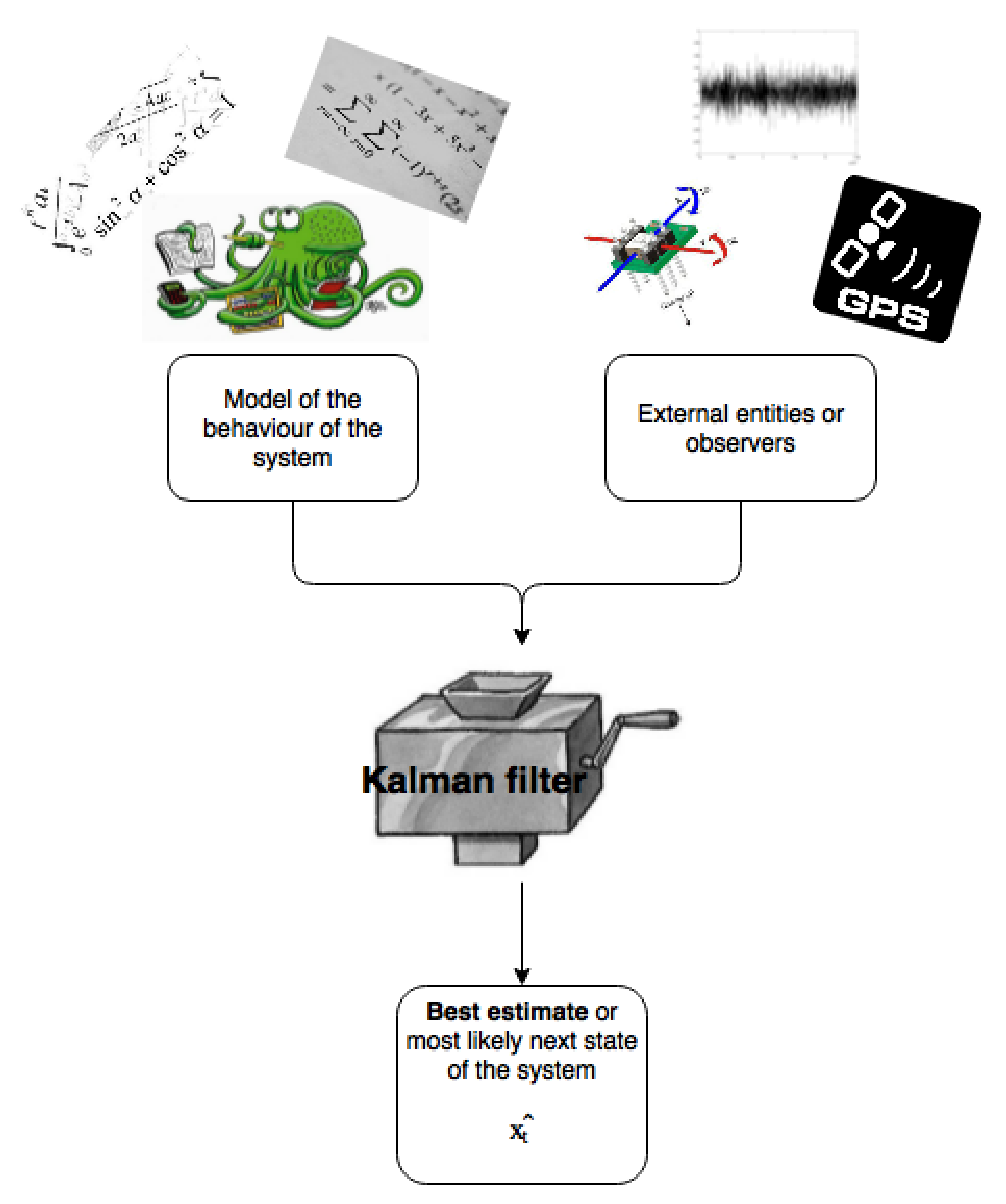
\includegraphics[width=0.75\textwidth]{kalman_input_output}
  \caption{The model and the observations go into the Kalman filter to
    get the best estimate for the next state of the system.}
  \label{fig:kalman_crank_machine}
\end{figure}

In case that your model is incomplete, it means there are factors you
did not know how to include in your model (or you did not even have
idea they exist), you should have no worries. The Kalman filter will
try to introduce them for you. However, if the behaviour of your
system cannot be described as a linear process or the error introduced
by your model or the lectures from the external observers do not
follow a Gaussian distribution, then the Kalman filter may not be what
you are looking for. In this case check for \textit{modified} versions
of the filter such as the extended Kalman filter \cite{} or the
Unscented Kalman filter \cite{}.

\subsection{Thinking Bayesian}
If you have not yet got the idea of the Kalman filter, think of it as
an special case of a Bayesian filter:
\begin{equation}
  \label{eq:bayesian}
  P(H|D) = \frac{P(H) \times P(D|H)}{P(D)}
\end{equation}
where
\begin{itemize}
\item $P(H|D)$, is the probability of the hypothesis $H$ given the
  data $D$,
\item $P(H)$, is the probability of the hypothesis $H$,
\item $P(D|H)$, is the probability of the data $D$ given the
  hypothesis $H$,
\item $P(D)$, is the probability of the data $D$.
\end{itemize}
Thus the Kalman filter is as follows:
\begin{equation}
  \label{eq:kalman_as_bayesian}
  P(H_t|H_{t-1},A_t,D_t)
\end{equation}
which states for the probability of the hypothesis $H_t$ at time $t$
\textbf{given} the hypothesis $H_{t-1}$ at time $t-1$, the action $A$
taken at time $t$, and the data $D_t$ at time $t$.

\subsection{Predict and update}
The Kalman filter has got two general stages:
\begin{enumerate}
\item The \textit{prediction stage}, where the next state of the
  system is obtained using a \textbf{model}. This model describes the
  change of state of the system. It can be \textbf{a mathematical
    model} or a set of data where we can look for the next state of
  the system given the current state.
\item The \textit{updating stage}, where \textit{the best} next
  possible state of the system is computed. This next stage is
  obtained by \textbf{combining} the information given by \textbf{the
    model} and the information provided by external entities or
  observers of the system. Examples of these external entities may be
  \textbf{sensors}.
\end{enumerate}

\subsection{The maths}
\label{sec:the_maths}
Do not be afraid of what follows, but here it is, the mighty,
glorious, and mostly feared: the \textbf{Kalman filter}.

\begin{align}
  \vect{x}_{t|t-1} &= F_t \vect{x}_{t-1|t-1} + B_t \vect{u}_t \label{eq:K1}\\
  P_{t|t-1} &= F_t P_{t-1|t-1} F_t^T + Q_t \label{eq:K2}\\
  \vect{x}_{t|t} &= \vect{x}_{t|t-1} + K_t (\vect{z}_t - H_t \vect{x}_{t|t-1}) \label{eq:K3}\\
  P_{t|t} &= P_{t|t-1} - K_t H_t P_{t|t-1} \label{eq:K4}
\end{align}
where
\begin{equation}
  \label{eq:K}
  K_t= P_{t|t-1} H_t^T (H_t P_{t|t-1} H_t^T+R_t)^{-1}
\end{equation}
As I mentioned before, do not freak out, when you end up reading this
document you will know what each term in these equations means. By
now, let us mention that \eqref{eq:K1} and \eqref{eq:K2} correspond to
\textbf{the prediction stage}, while \eqref{eq:K3} and \eqref{eq:K4}
correspond to \textbf{the updating stage}.

Equation \eqref{eq:K1} is used as the model that predicts the next
stage of our system based on the information we have on the previous
time ($t-1$). Equation \eqref{eq:K2} is the prediction of the
covariance matrix using the information from previous time and
considering some uncertainty on our model.

Equation \eqref{eq:K3} obtains the best estimate for $\vect{x}_{t|t}$
(the state of the system), it considers the predicted value of
$\vect{x}_{t|t-1}$ and the measurements of the sensors. Equation
\eqref{eq:K4} is in charge of updating the covariance matrix based on
the predicted values of the same matrix. Equation \eqref{eq:K}
provides the fusion of the information, the $K_t$ matrix is called
\textbf{the Kalman gain}.

Now check and try to find a correspondence between equations
\eqref{eq:K1}, \eqref{eq:K2}, \eqref{eq:K3}, \eqref{eq:K4} and
\eqref{eq:K} in Figure \ref{fig:kalman_workflow}, which shows the
general work flow of the Kalman filter with its inputs and outputs.
\begin{figure}
  \centering
  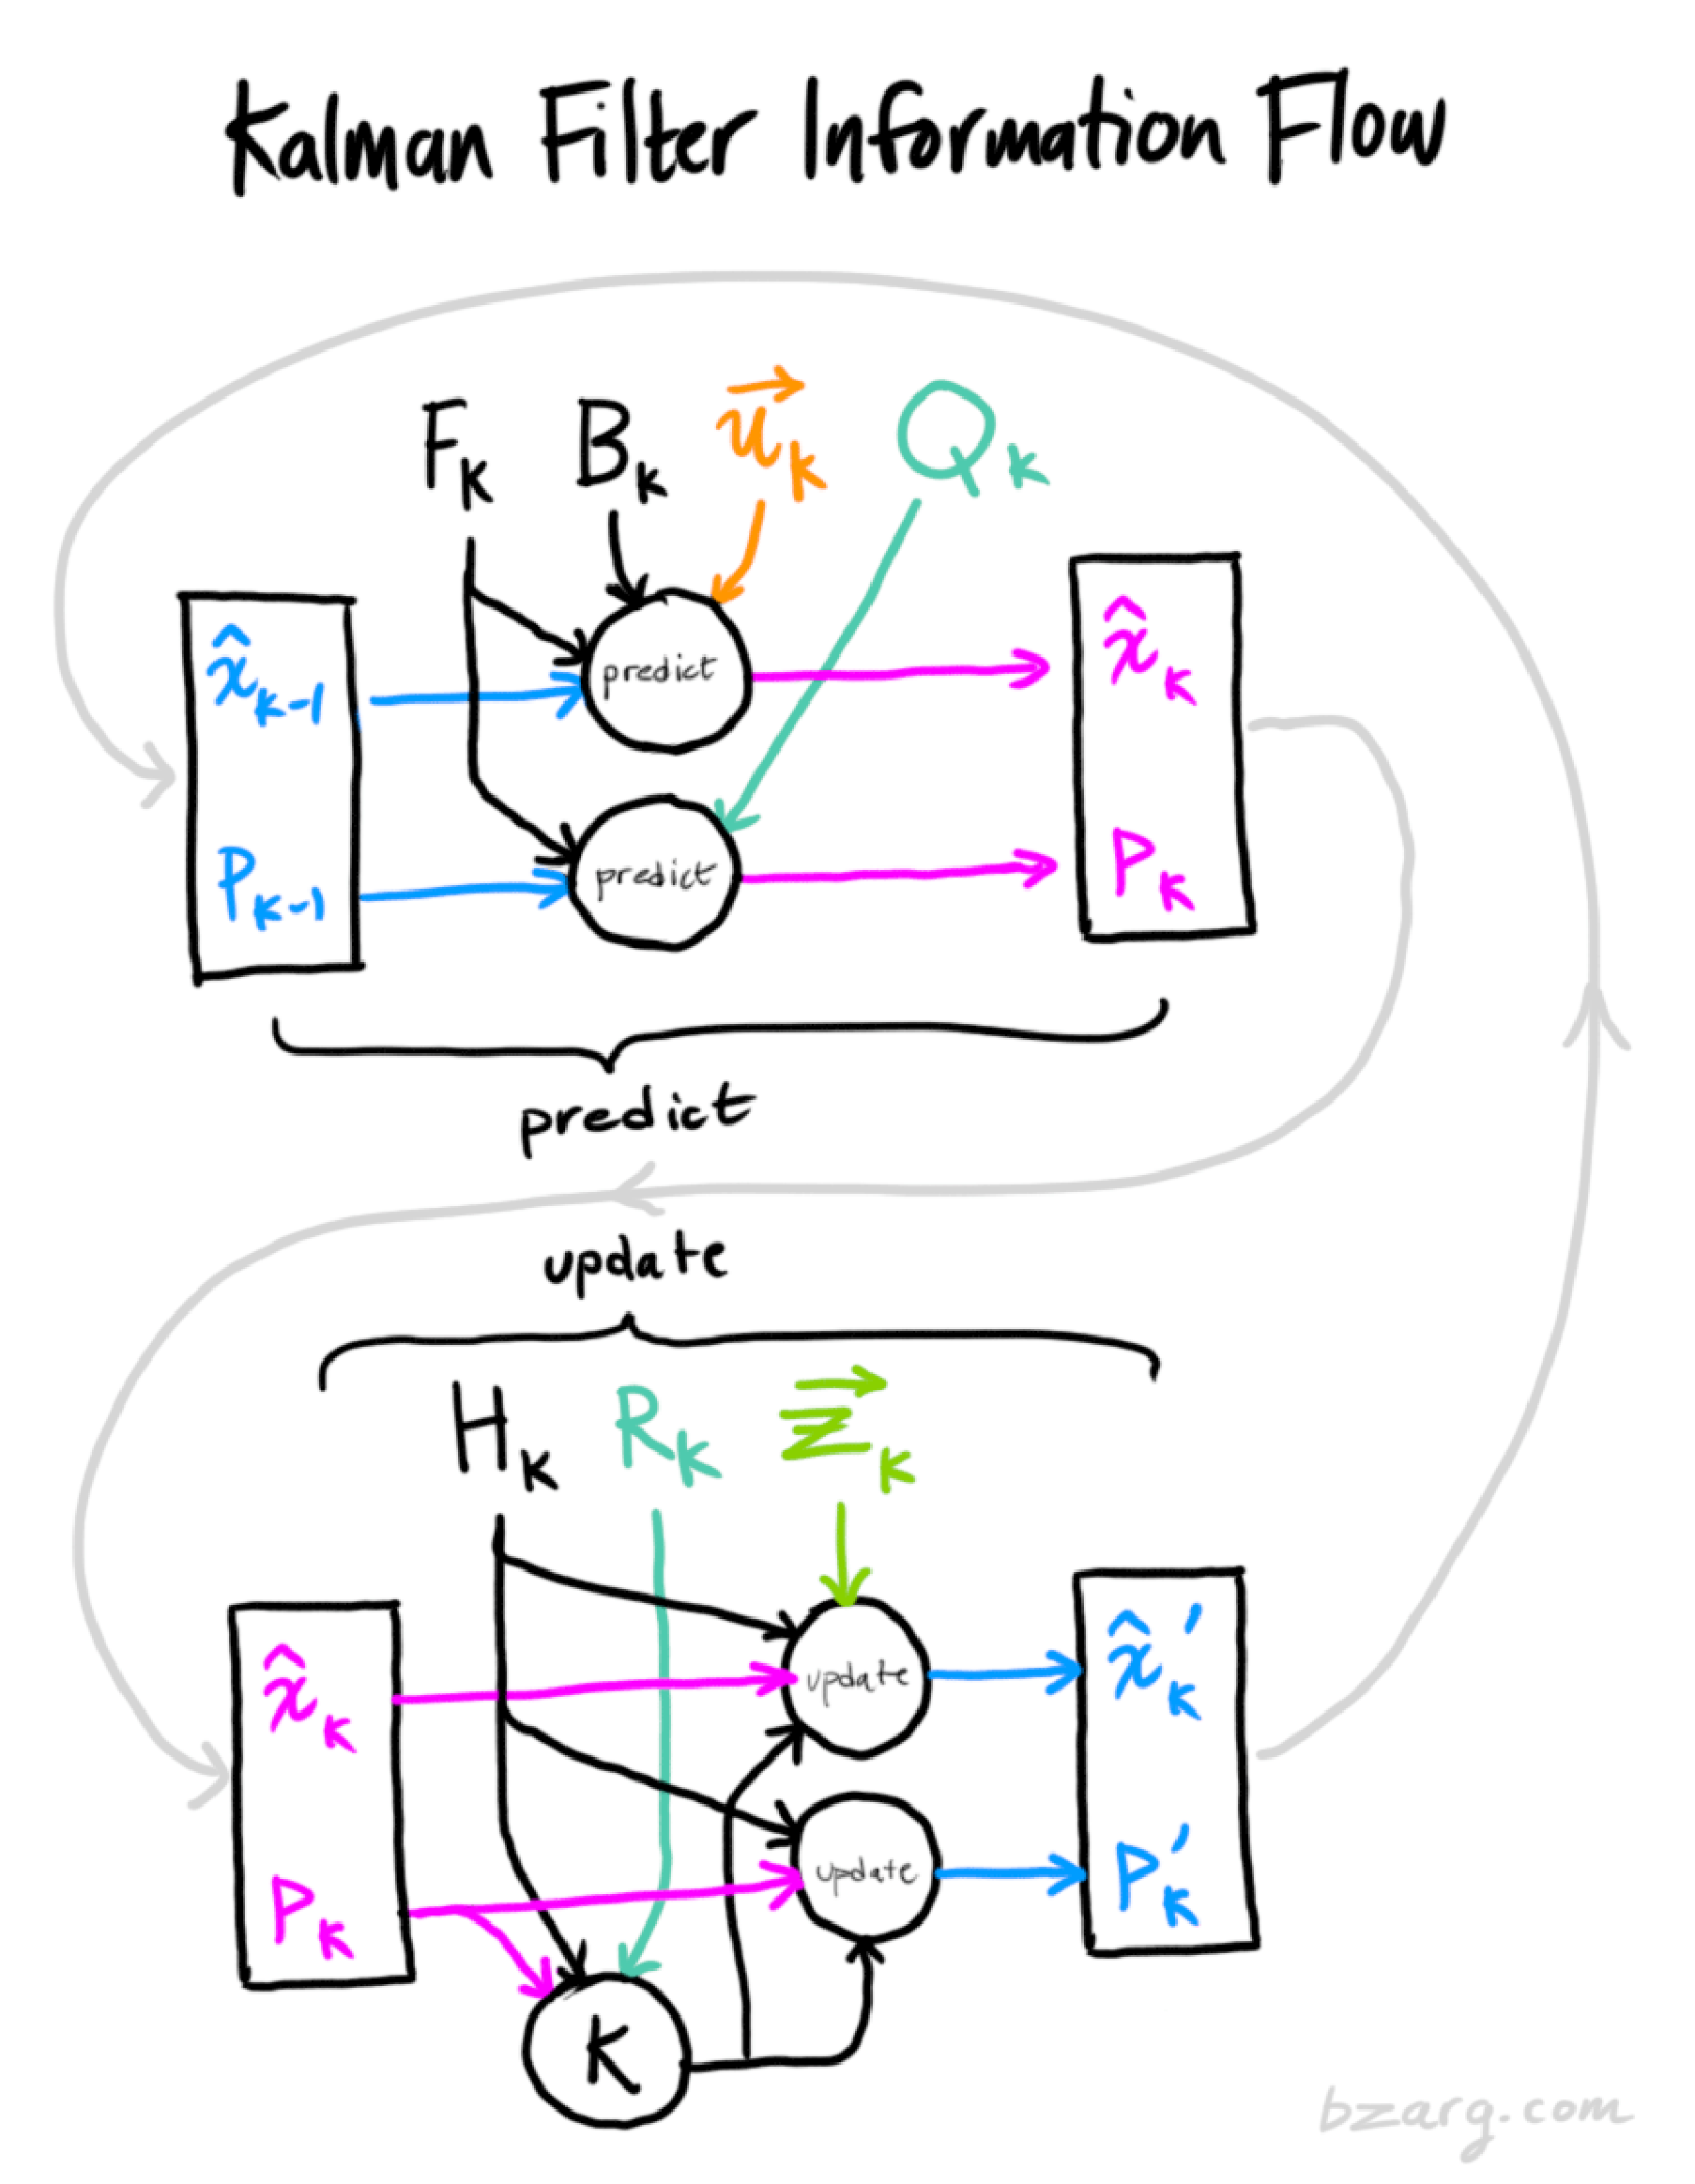
\includegraphics[width=1.0
 \textwidth]{kalflow}
 \caption{Work flow of Kalman filter showing the input/output
   variables. Taken from \cite{Bzarg:2011:URL}}
  \label{fig:kalman_workflow}
\end{figure}

The Kalman filter incorporates the prediction from a model and the
prediction of sensors based on the model with the actual reading of
the sensors to get a better estimate of the next state of the system.

\section{A simple example: a moving object in 1D}
\label{sec:example1D}
Here we present an example to predict the position of an object that
moves along one direction, see Figure \ref{fig:object_1D_00}.
\begin{figure}
  \centering
  \includegraphics[width=1.0\textwidth]{object_1D_00}
  \caption{An object moving along one direction. Taken from
    \cite{Faragher:2012:ARTICLE}.}
  \label{fig:object_1D_00}
\end{figure}

\subsection{The mathematical model}
We can describe the position and the velocity of an object as follows:
\begin{align}
  p_t &= p_{t-1} + v_{t-1} t + \frac{1}{2} a_t t^2 \label{eq:object_position_1D}\\
  v_t &= v_{t-1} + a_{t} t \label{eq:object_velocity_1D}
\end{align}
where $p_t$ and $v_t$ are the position and the velocity of the object
at time $t$, respectively. The coefficient $a_t$ represents the
acceleration of the object at time $t$.

Re-writing \eqref{eq:object_position_1D} and
\eqref{eq:object_velocity_1D} as one equation using matrix notation we
have:
\begin{equation}
  \label{eq:one_d_matrix_form}
  \vect{x}_t = F_t \vect{x}_{t-1} + B_t \vect{u}_t
\end{equation}
where
\begin{align}
  \vect{x}_t =
  \begin{bmatrix}
    p_t \\
    v_t
  \end{bmatrix}
  \quad
  F_t =
  \begin{bmatrix}
    1 & t\\
    0 & 1
  \end{bmatrix}
  \quad
  \vect{x}_{t-1} =
  \begin{bmatrix}
    p_{t-1} \\
    v_{t-1}
  \end{bmatrix}\\
  B_t = 
  \begin{bmatrix}
    \frac{t^2}{2} \\
    t
  \end{bmatrix}
  \quad
  \vect{u}_t =
  \begin{bmatrix}
    a
  \end{bmatrix}
\end{align}

\begin{itemize}
\item $\vect{x}_t$ is the state vector, containing the variables that
  describe our system,\\
\item $F_t$ is the state transition matrix, which applies the effect
  of the variables at time $t-1$ to obtain the system state at time $t$\\
\item $\vect{u}_t$ is the control input vector, which includes noisy
  information to our system,
\item $B_t$ is the control input matrix, which applies the effect of
  the control input vector on the state vector.\\
\end{itemize}

Note that \eqref{eq:one_d_matrix_form} looks quite similar to
\eqref{eq:K1}, the first equation of the Kalman filter. Indeed,
\eqref{eq:one_d_matrix_form} is the \textbf{mathematical model} that
describes the behaviour of our system. The differences between
\eqref{eq:one_d_matrix_form} and \eqref{eq:K1} comes from the not so
friendly notation used to describe the equations of the Kalman filter,
but let us try to explain it here.

The first step into understanding the equations that make the Kalman
filter is to understand its notation, thus every time you see
$\vect{x}_{t|t-1}$, you should read it as the value of $\vect{x}$
computed at time $t$ using information at time $t-1$. This way
\eqref{eq:K1} obtains a \textit{prediction} of $\vect{x}$ at time $t$
using information at time $t-1$. The same happens with \eqref{eq:K2}
which is a \textit{prediction} of the covariance matrix $P$ at time
$t$ using information at time $t-1$.

\subsection{The covariance matrix}
The uncertainty on the state of the system is represented by a
covariance matrix $P_t$. The Kalman filter uses covariances instead of
only variances to model the relations between variables. These
relations are introduced in the off-diagonals of the covariance
matrices.

In our 1D example we are working with only two variables, namely,
position $p$ and velocity $v$, thus our covariance matrix for the
\textit{prediction} stage is a $2 \times 2$ matrix given as follows:
\begin{equation}
  \label{eq:covariance_Q}
  P_t =
  \begin{bmatrix}
    \sigma_p^2 & \sigma_{p}\sigma_{v} \\
    \sigma_{v}\sigma_{p} & \sigma_v^2
  \end{bmatrix}
\end{equation}
You should read this matrix as follows: the entries at the diagonal
represent the influences of the variables over themselves. The
off-diagonals are the influences of the variable at row $i$ and column
$j$. If we assume that in our 1D example the variances in our states
are given by the control inputs, that is, the acceleration terms, thus
we have:
\begin{align}
  \label{eq:covarianve_1D_example}
  P_t &=
        B_t B_t^T\\
      &= 
        \begin{bmatrix}
          \frac{t^2}{2} \\
          t
        \end{bmatrix}
        \begin{bmatrix}
          \frac{t^2}{2} & t\\
        \end{bmatrix}\\
      &=
        \begin{bmatrix}
          \frac{t^4}{4} & \frac{t^3}{2}\\
          \frac{t^3}{2} & t^2
        \end{bmatrix}
\end{align}

From the covariance matrix we obtain the process noise covariance
matrix $Q_t$ which for our example is initialised as follows:
\begin{equation}
  \label{eq:noise_Q}
  Q_t = \sigma_a^2 P_0.
\end{equation}

\subsection{Updating the state using sensors measurements}
The initial stage of the system is known, for our case we know the
position and the initial velocity of the object, see Figure
\ref{fig:object_1D_01}.
\begin{figure}
  \centering
  \includegraphics[width=0.75\textwidth]{object_1D_01}
  \caption{The initial state of the object with a normal probability
    density function representing the \textit{initial} confidence on
    the estimation of the position. Taken from
    \cite{Faragher:2012:ARTICLE}.}
  \label{fig:object_1D_01}
\end{figure}

Now that we are able to predict the state of our system using
\eqref{eq:K1}, and we can also predict our new uncertainty using
\eqref{eq:K2}, we will \textbf{combine} these \textit{predictions}
with actual sensors readings to get a \textbf{better} estimate of the
next state of the system, see Figures \ref{fig:object_1D_02} and
\ref{fig:object_1D_03}.

\begin{figure}
  \centering
  \includegraphics[width=0.75\textwidth]{object_1D_02}
  \caption{We can predict the new position of our object, and the new
    uncertainty. Note that the uncertainty has increased due to
    influences of the external world that we are not accounting for in
    our model.Taken from \cite{Faragher:2012:ARTICLE}.}
  \label{fig:object_1D_02}
\end{figure}

\begin{figure}
  \centering
  \includegraphics[width=0.90\textwidth]{object_1D_03}
  \caption{We got two estimations for the position of our object; the
    first one based on a mathematical model, and the second one based
    on the actual readings of the sensors. Taken from
    \cite{Faragher:2012:ARTICLE}.}
  \label{fig:object_1D_03}
\end{figure}

\subsubsection{The not always square matrix $H_t$}
We first need to define the matrix $H_t$, which applies a
transformation from the prediction domain to the measurement
domain.\footnote{Remember that the prediction is obtained from a
  mathematical model.} Think of this matrix as an auxiliary matrix
that helps you to transform between the units used in the vector state
$\vect{x}_t$ to the units used by the sensors.\footnote{For example,
  to transform from metres to kilometres.}

In our 1D example, we assume that the mathematical model and the
sensors \textit{talk} the same language, thus we need to indicate that
in the $H_t$ matrix. Additionally, we may find that the sensors do not
provide measurements for all the variables in our model (position and
velocity), thus we need to restrict our transformation matrix to work
only with the measures provided by the sensors. This is the reason why
the $H_t$ matrix is not always square.

Since we are working with two variables and lets say that our sensors
only give us the position then the transformation matrix for our
example is as follows:
\begin{equation}
  \label{eq:transformation_matrix}
  H_t = 
  \begin{bmatrix}
    1 & 0
  \end{bmatrix}
\end{equation}

\subsubsection{Combining the information using the Kalman gain}
Now it is time to define some stuff in \eqref{eq:K3}, there we have
the vector $\vect{z}_t$ which represents the actual readings of the
sensors. We want to know how good is our prediction compared with the
actual sensor reading. Mathematically, this is expressed by
\begin{equation}
  \label{eq:diff_sensor_prediction}
  \vect{d}_t = \vect{z}_t - H_t \vect{x}_{t|t-1}
\end{equation}

In order to combine the information obtained by the mathematical model
and the actual readings of the sensors we need to consider their
uncertainties in the prediction and the sensors measurements. These
uncertainties are represented by normal distributions around the
predicted and measured states of the system (position of the object in
our example), see Figure \ref{fig:object_1D_03} again. We perform the
\textbf{fusion} of the information by \textbf{multiplying} both
distributions, see Figure \ref{fig:object_1D_04}.

\begin{figure}
  \centering
  \includegraphics[width=0.90\textwidth]{object_1D_04}
  \caption{Fusion of information by multiplying both
    distributions. From the obtained distribution (the green one) we
    get a better estimate for the state of the system. Taken from
    \cite{Faragher:2012:ARTICLE}.}
  \label{fig:object_1D_04}
\end{figure}

The multiplication of the distributions is given by \eqref{eq:K},
which we rewrite here
\begin{equation}
  \label{eq:K_again}
  K_t= P_{t|t-1} H_t^T (H_t P_{t|t-1} H_t^T+R_t)^{-1}
\end{equation}
where $R_t$ is a matrix representing the noise in the measurement of
the sensors. Note that the larger the noise, the smaller the Kalman
gain, and \textit{vice versa}. Think of the Kalman gain as a measure
of information, the less informative (or more noisy) are the
measurements of the sensors then the less informative becomes the
Kalman gain. The more informative, or trusted, are the measurements of
the sensors, the more trusted is the Kalman gain.

Note that in order to equation \eqref{eq:K_again} \textit{makes
  sense}, $dim(R_t)$ must be equal to $dim(H_t P_{t|t-1} H_t^T)$. The
matrices $H_t$ and $H_t^T$ act like some sort of \textit{permutation}
matrices. In our specific problem, multiplying from right to left,
$H_t P_{t|t-1} H_t^T$ tell us to take the elements in the first column
and then the elements in the first row, the result is a $1 \times 1$
matrix which must match the dimension of the $R_t$ matrix. The matrix
$R_t$ is as follows:
\begin{equation}
  \label{eq:noise_measurements}
  R_t = 
  \begin{bmatrix}
    \sigma_z^2
  \end{bmatrix}
\end{equation}

Thus, we are going to \textbf{update} our predictions based on:
\begin{itemize}
\item how trusted the measurements of our sensors are,
\item how different are the data obtained from our model and the
  actual sensor readings
\end{itemize}
We already have those two ingredients, lets put them together:
\begin{align}
   \vect{x}_{t|t} &= \vect{x}_{t|t-1} + K_t (\vect{d}_t) \label{eq:K3_again}\\
   P_{t|t} &= P_{t|t-1} - K_t H_t P_{t|t-1} \label{eq:K4_again}
\end{align}
If you did not noticed it, \eqref{eq:K3_again} is a simplified version
of \eqref{eq:K3}, we just plugged in the vector $\vect{d}_t$ from
\eqref{eq:diff_sensor_prediction} instead of explicitly writing the
difference between the prediction and the actual sensors
readings. Thus, \eqref{eq:K3_again} performs an update on the state of
the system using the current estimation and adding the weighted
difference (by the Kalman gain) between the state prediction and the
actual sensors readings. Equation \ref{eq:K4_again} is in charge of
updating the covariance matrix using the current estimation and
subtracting the weighted estimation mapped to the sensors domain.

Now go back to section \ref{sec:the_maths} and read through it
again. Once you are done, jump into the next section.

\subsection{Implementation}
We present a simple implementation based on the mathematical model,
covariance and transformation matrices presented in the previous
sections. The implementation is based on the software library
\texttt{OpenCV} \cite{opencv:2000:ARTICLE}. In order to match and ease
the use of the Kalman filter implemented in that library, we created a
wrapper class such that the notation in the implementation follows the
one presented in the previous sections.

\subsubsection{C++ wrapper class}
We created the class \texttt{CCKalmanFilter} which is a wrapper to
\texttt{OpenCV}'s Kalman filter implementation


n summary, we got our mathematical model

\section{Another (also simple) example: a moving object in 2D}
\label{sec:example2D}


\section{Implementations of the Kalman filter}
We use \texttt{OpenCV} \cite{opencv:2000:ARTICLE} implementation of
the Kalman filter

\section{Conclusions}

% ========================================================================
% Customising bibliography ------------------- BEGIN ---------------------
% ========================================================================
\printbibliography[heading=bibintoc]
% Print bibliography from articles
%\printbibliography[heading=bibintoc, type=article,title={Articles}]
% Print bibliography from books
%\printbibliography[heading=bibintoc,type=book,title={Books}]
% Print bibliography from incollection
%\printbibliography[heading=bibintoc,type=incollection,title={In collection}]
% ========================================================================
% Customising bibliography ------------------- END -----------------------
% ========================================================================

\end{document}
